%\vfill\eject
\section{Preliminary}
\label{sec:framework}

The framework of the taxonomy based code mining system can be divided into two main
parts, topic mining and taxonomy mapping. Topic mining aims to mine the topic
distributions of code files.
\begin{table}[h]
\centering
\label{tab:anno}
\begin{tabular}{|c|c||c|c||c|c|}
\hline
Symbol & Def & Symbol & Def & Symbol & Def\\\hline \hline
$Z$ & topic & $Z$ & topic & $D$ & file \\\hline
$Z$ & topic & $w$ & word & $C$ & commit \\\hline
$Z$ & topic & $a$ & connection & l & language \\\hline
\end{tabular}
\caption{All Symbols Used in Paper}
\end{table}

\subsection{Repository Corpus}
\label{sec:repo}
A repository is a concept from revision control that refers to a data structure,
usually stored on a server, that contains, among other things:
\begin{itemize}
\item A set of files and directories.
\item Historical record of changes in the repository.
\item A set of commit objects.
\item A set of references to commit objects, called heads.
\end{itemize}
A code repository contains many source code files, configuration files and usually
the commit messages during the generation of it.
The data contained in code repositories are not ``plain'', a
code file consists codes which may be decided by programming
languages and natural language comments which is written by the programmers.
We try to design one probabilistic graphical model to mine knowledge from
repositories which can take advantages of the structure information of them.

According to the special features of code files, they are usually hard to understand
by human directly. Unfortunately there is also not a labeled code dataset for us. 

Source code are developed by programmers. They used to
denote variables and function names with ``meaningful'' words. And plenty of comments
are telling readers what this code is about. In addition, the commit information created
during the process of development also provide some help to understand the code.


\subsection{Taxonomy}
\label{sec:taxonomy}
The famous programming Q\&A website Stackoverflow have more than 37 thousands
tags. A folksonomy is a system of classification derived from the practice and
method of collaboratively creating and translating tags to annotate and categorize
content; this practice is also known as collaborative tagging, social classification,
social indexing, and social tagging.  This is a liner structure taxonomy.

The ACM Computing Classification System\cite{acmurl} is a subject classification
system for computing devised by the Association for Computing Machinery. This
classification system contains a six-level tree with totally more than 2000 nodes.
Higher levels of the tree are usually more generous, one node is a sub-area of its
parents.
\figref{fig:acm} shows a subtree ``Contextual software domains''of the
classification system.
\begin{figure}[h]
\begin{center}
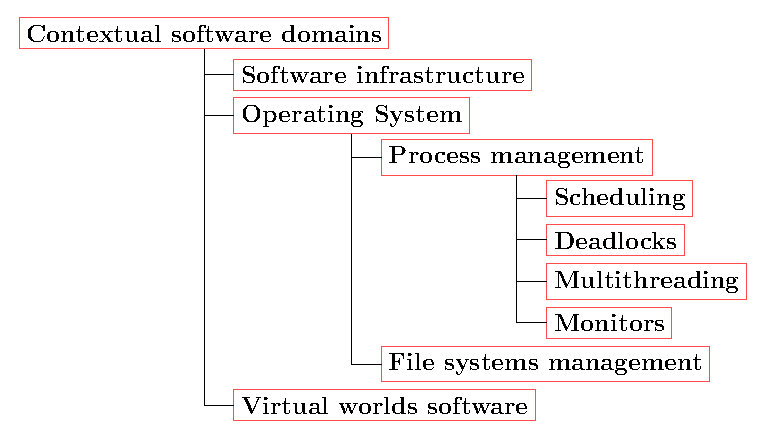
\includegraphics[width=0.9\columnwidth]{figure/acm.eps}
\caption{ACM Computing Classification System}
\label{fig:acm}
\end{center}
\end{figure}

The ACM Computing Classification System provides us a framework of the
taxonomy. We build the context for each node of it by searching the
corresponding concepts pages from Wikipedia.
